\newpage
\section{Cel ćwiczenia}

Celem zajęć było zbudowanie uproszczonego układu sterowania trzema podajnikami taśmowymi pracującymi w jednym ciągu. Program napisaliśmy w języku drabinkowym w LOGO! Soft Comfort i sprawdziliśmy go w symulacji sterownika Siemens.

Układ ma działać tak, że po naciśnięciu START najpierw rusza podajnik 1. Podajnik 2 włącza się dopiero po zadanym opóźnieniu względem pierwszego, a podajnik 3 po kolejnym opóźnieniu względem drugiego. Dzięki temu materiał nie spada na jeszcze stojącą taśmę. STOP zatrzymuje cały ciąg w dowolnej chwili, a po zaniku i powrocie zasilania podajniki same się nie uruchamiają.

Druga część programu dotyczy odporności na awarie. Każdy podajnik ma własny sygnał awarii. Awaria odcina dany napęd i podajniki, które od niego zależą: awaria pierwszego zatrzymuje cały ciąg, awaria drugiego zatrzymuje drugi i trzeci, awaria trzeciego zatrzymuje tylko trzeci. Następny podajnik może pracować tylko wtedy, gdy pracuje poprzedni.

Po ćwiczeniu potrafimy:

\begin{itemize}
    \item przypisać przyciski, styki awaryjne i napędy do wejść i wyjść sterownika LOGO!,
    \item zapisać rozruch trzech podajników z dwoma niezależnymi opóźnieniami,
    \item podtrzymać stan pracy na markerze i zdjąć go przyciskiem STOP oraz po zaniku zasilania,
    \item odciąć uszkodzony podajnik i zależne od niego odcinki na podstawie styków awaryjnych,
    \item sprawdzić sekwencję, opóźnienia i reakcję na awarie w symulatorze.
\end{itemize}

\section{Stanowisko}

Do pracy użyliśmy komputera z zainstalowanym LOGO! Soft Comfort oraz Siemens. Program rysowaliśmy jako schemat drabinkowy, nastawy timerów i przypisanie wejść sprawdzaliśmy najpierw w symulacji, a następnie na samym sterowniku.

Przypisanie sygnałów, do którego doszliśmy w końcowej wersji programu, zebraliśmy w tabeli~\ref{tab:io}.

\begin{table}[h]
    \centering
    \caption{Wejścia i wyjścia użyte w programie}
    \label{tab:io}
    \begin{tabular}{|l|l|p{8.5cm}|}
        \hline
        \textbf{Adres} & \textbf{Element} & \textbf{Rola} \\
        \hline
        I1 & przycisk START & impuls załączenia układu \\
        \hline
        I2 & przycisk STOP & zatrzymanie i zdjęcie podtrzymania \\
        \hline
        I3 & awaria napędu 1 & styk wyłącznika silnikowego \\
        \hline
        I4 & awaria napędu 2 & styk wyłącznika silnikowego \\
        \hline
        I5 & awaria napędu 3 & styk wyłącznika silnikowego \\
        \hline
        Q1 & napęd 1 & pierwszy podajnik taśmowy \\
        \hline
        Q2 & napęd 2 & drugi podajnik taśmowy \\
        \hline
        Q3 & napęd 3 & trzeci podajnik taśmowy \\
        \hline
        M1 & marker & pamięć stanu „układ załączony” \\
        \hline
        T1, T2 & timery & odstępy między kolejnymi rozruchami \\
        \hline
    \end{tabular}
\end{table}

\begin{figure}[H]
    \centering
    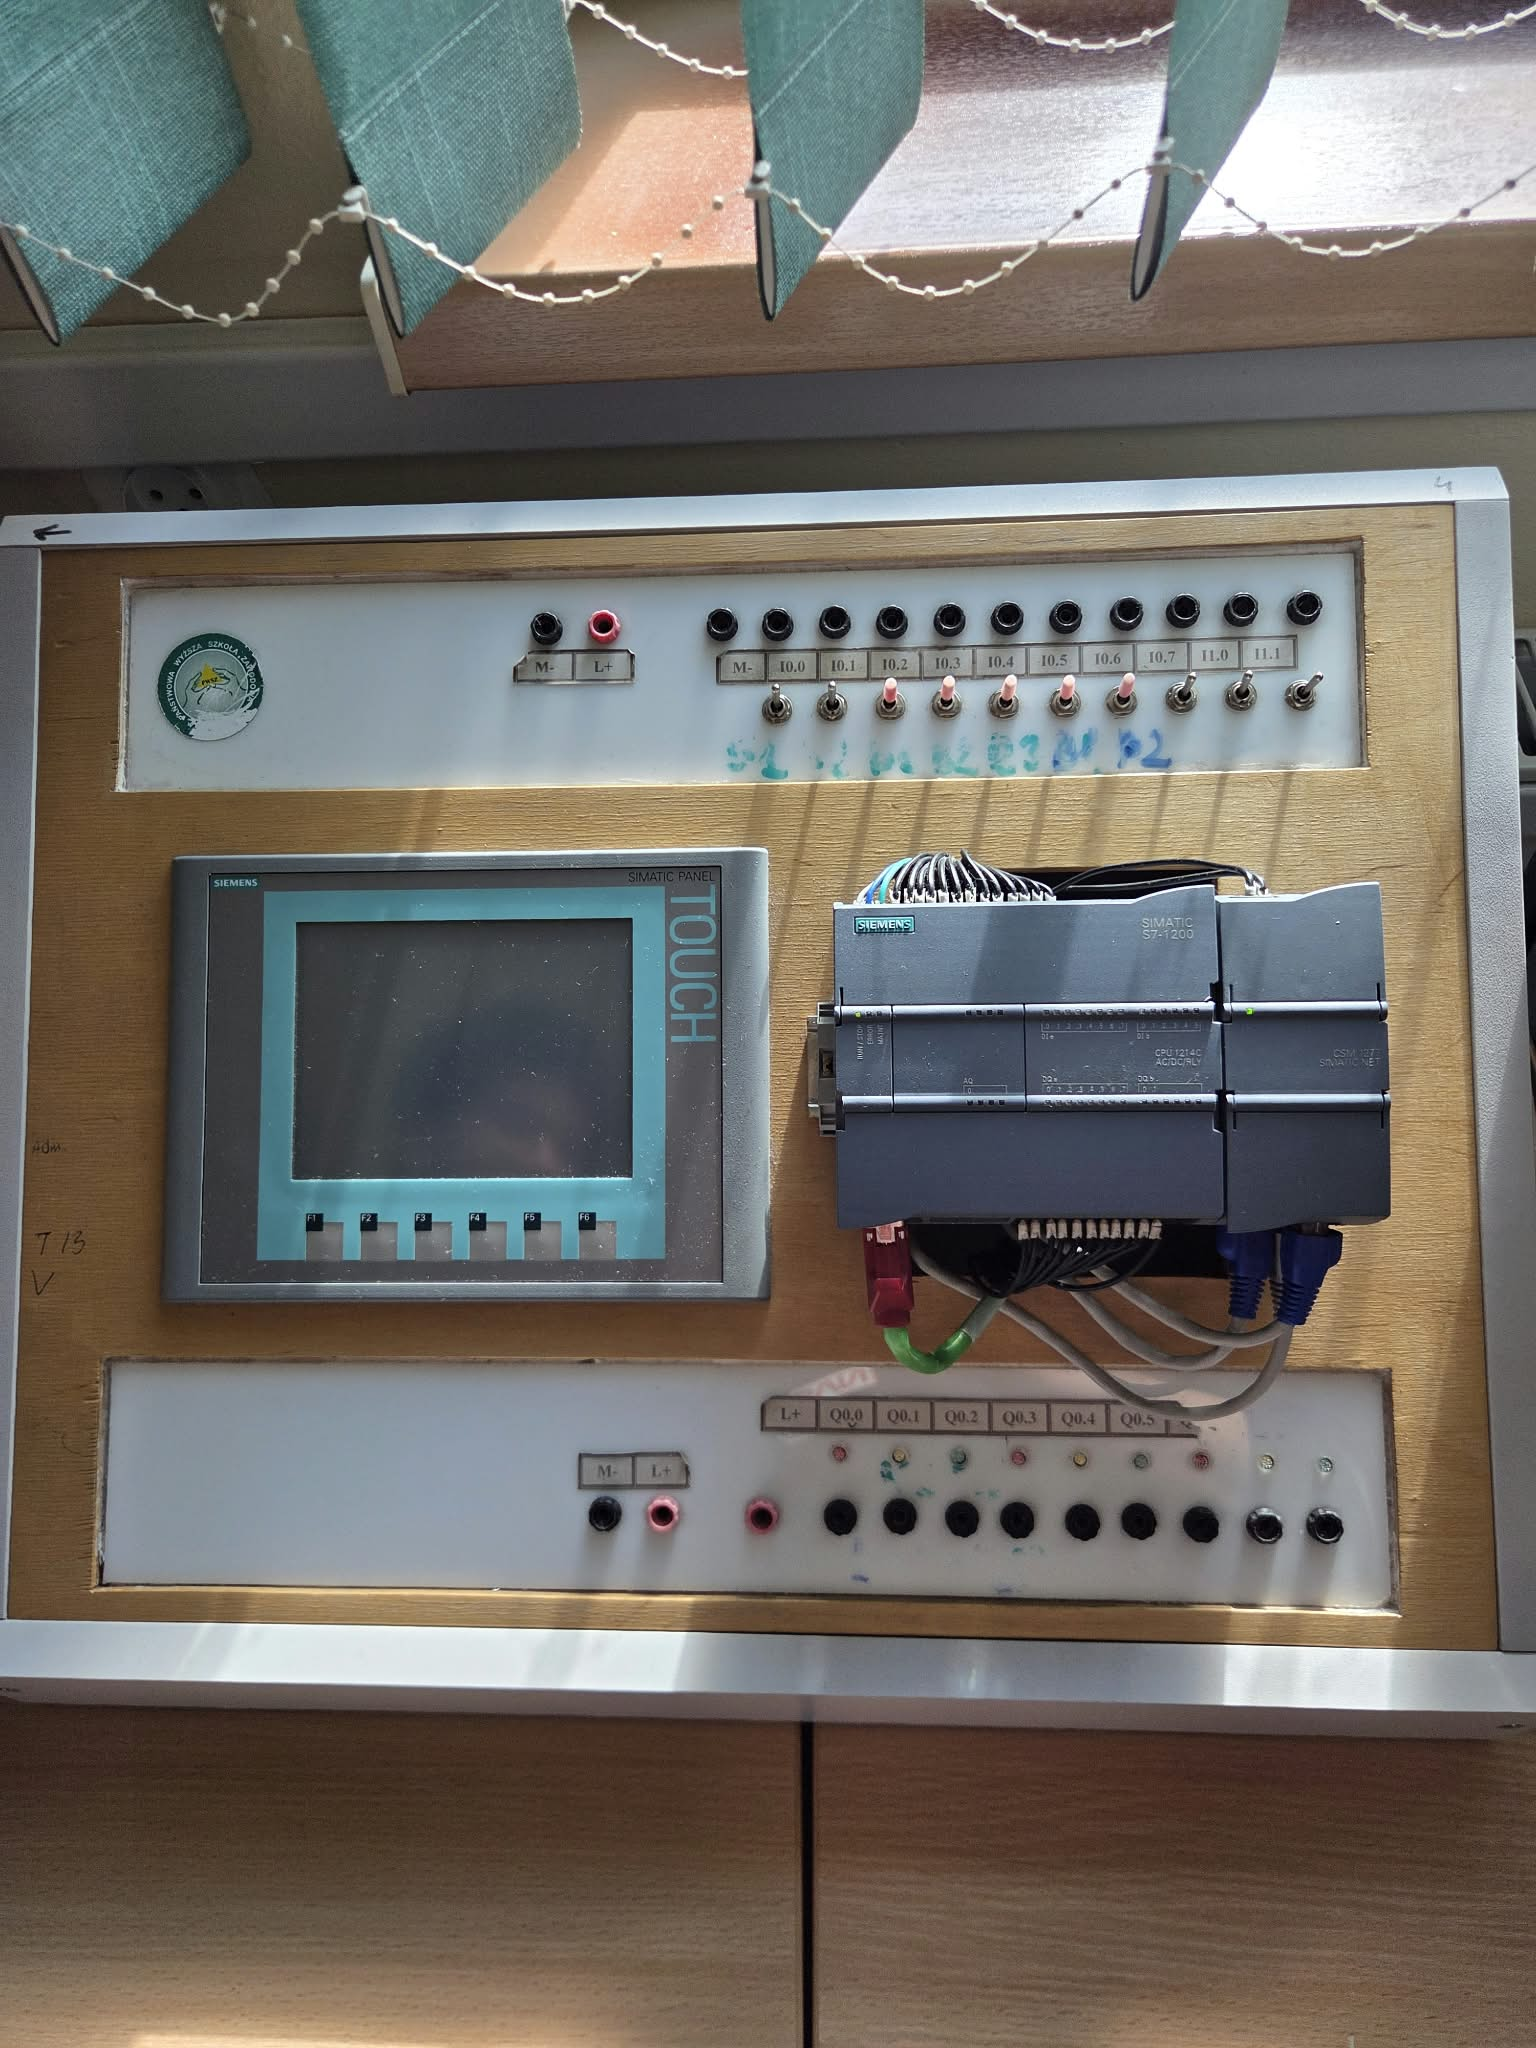
\includegraphics[width=0.45\textwidth]{rys/simens.jpeg}
    \caption{Stanowisko ze sterownikiem Siemens LOGO!}
    \label{fig:stanowisko}
\end{figure}

\begin{figure}[H]
    \centering
    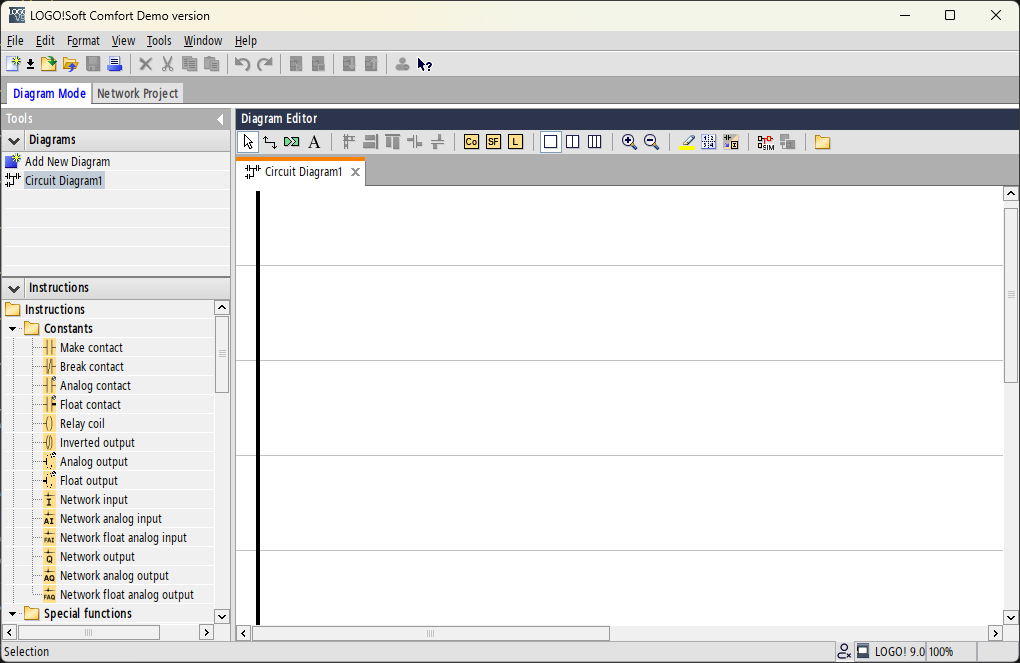
\includegraphics[width=0.85\textwidth]{rys/logo.png}
    \caption{Okno projektu w LOGO! Soft Comfort}
    \label{fig:logo-soft}
\end{figure}
